%%
% Please see https://bitbucket.org/rivanvx/beamer/wiki/Home for obtaining beamer.
%%
\documentclass{beamer}
\usetheme{Warsaw}

\usepackage{blkarray}
\usepackage{bigstrut}
\usepackage{amsmath}
\usepackage{bbm}

\makeatletter
\let\BA@quicktrue\BA@quickfalse
\makeatother

\title{Higher Order Markov Chains and Spacey Walks}
\author{Nicolas Nytko}
\date{\today}

\begin{document}
\frame{\titlepage}

% Overview
\begin{frame}
  \frametitle{Overview}
  \begin{enumerate}
  \item Introduction/review of first-order Markov chains
  \item Higher order Markov chains, relation to tensors
  \item Stochastic walks on higher order Markov chains
  \item Applications of the Spacey walk
  \end{enumerate}
\end{frame}


% Review of first-order markov chains
\begin{frame}
\frametitle{Markov Chains}
{\bf Markov Chains} are stochastic models describing a sequence of states with a probability of transitioning between each.
\begin{itemize}
\item Defined as matrix: ${\bf P} \in \mathbb{R}^{n\times n}$, ${\bf P}_{ij}$ gives probability of moving to state $i$ from $j$, for chain with $n$ states.
\item Given distribution/state vector ${\bf x}^{(n)}$, one step of a random walk is represented by matrix-vector product ${\bf x}^{(n+1)} = {\bf P} {\bf x}^{(n)} \enskip \Leftrightarrow \enskip x^{(n+1)}_i = \sum_j P_{ij} x^{(n)}_j $.
\end{itemize}

\begin{block}{}
\begin{columns}
\begin{column}{0.5\linewidth}
\centering
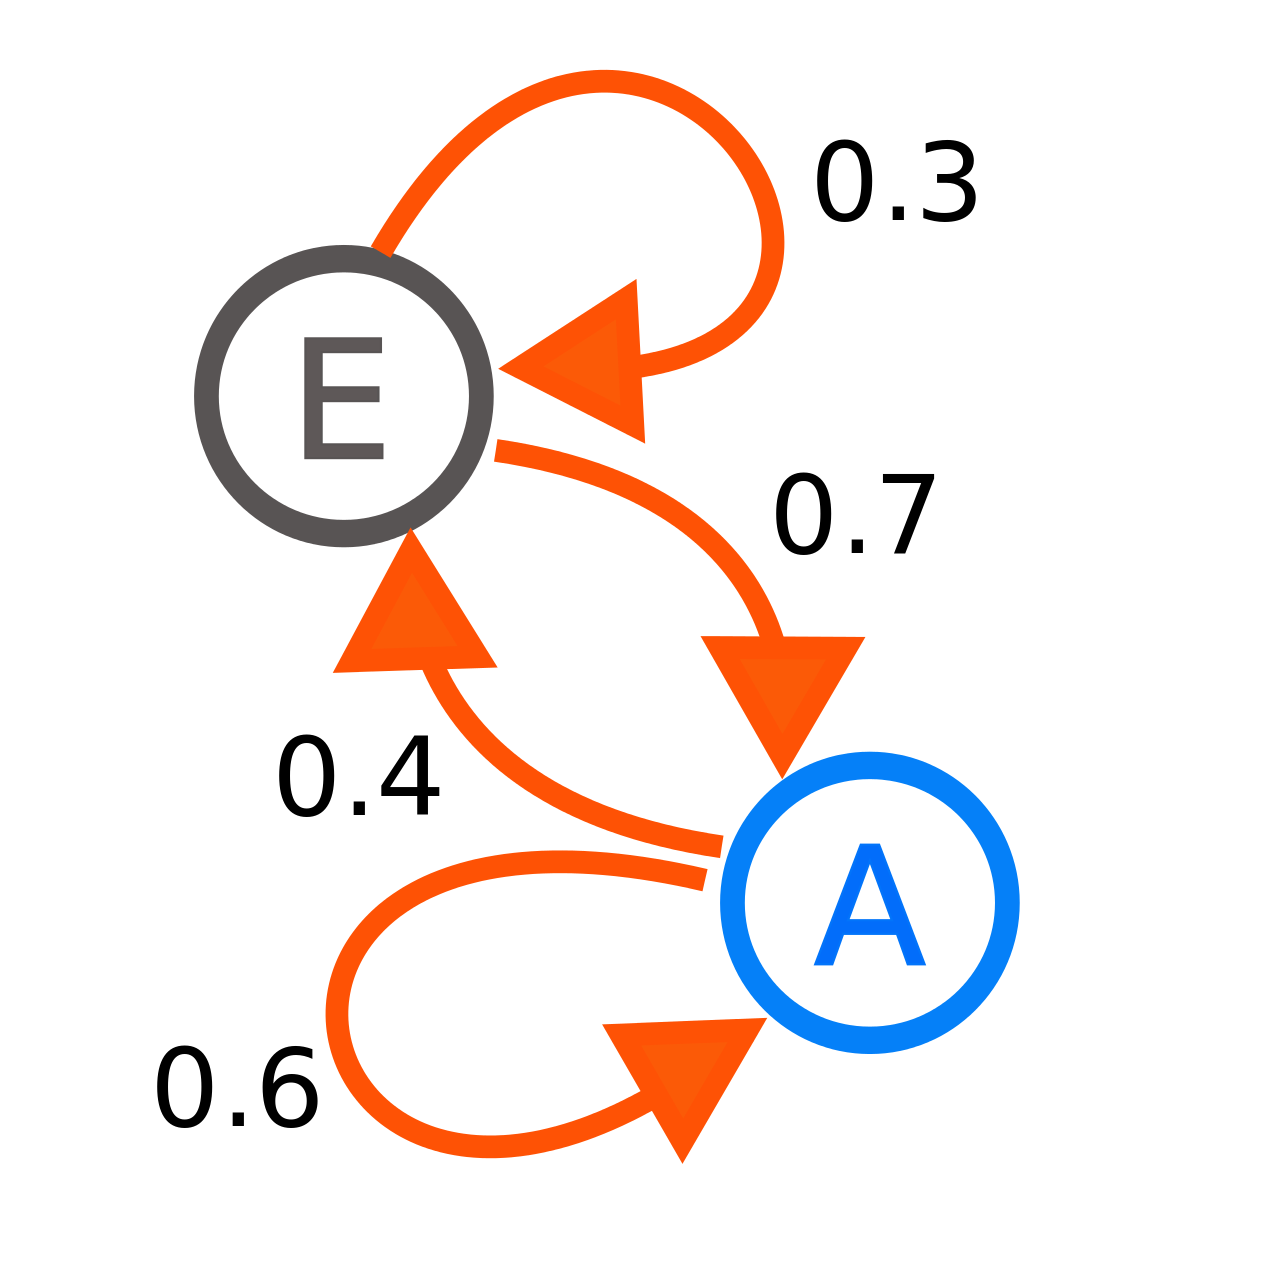
\includegraphics[scale=0.072]{images/markov.png}
\end{column}

\begin{column}{0.5\linewidth}
\centering
Transition matrix:
\[{\bf P} =
\begin{blockarray}{ccc}
  & A & E \\
	\begin{block}{c[cc]}
		\bigstrut[t]
		A & 0.6 & 0.7 \\
		E & 0.4 & 0.3
		\bigstrut[b] \\
	\end{block}
\end{blockarray}
\]
\end{column}
\end{columns}

\begin{center}
\begin{tiny}
Figure from \url{https://commons.wikimedia.org/wiki/File:Markovkate_01.svg}
\end{tiny}
\end{center}
\end{block}

\end{frame}


% Various definitions
\begin{frame}
\frametitle{Definitions}
\begin{block}{Time Homogeneous}
Each transition probability is independent of the time step $t$.
\end{block}

\begin{block}{Irreducible}
Every state can be reached from every other state.
\end{block}

\begin{block}{Periodic}
Periodic markov chain:
\[ \exists i \in S \quad s.t. \quad P_{ii} = 0\]
Periodicity implies a state may only return to itself after some multiple $d$ ``hops''.  If every state has self loops the chain is \textbf{aperiodic}.
\end{block}

\end{frame}


% Examples
\begin{frame}
\frametitle{Canonical Examples}

\textbf{Google PageRank}
\begin{itemize}
\item Markov chain represents the ``idealized'' web surfer.  States are webpages and transition probability is given by number of outgoing links between pages.
\item Ranking is determined by probability of being on certain page.
\end{itemize}

\textbf{Board Games}
\begin{itemize}
\item Each spot on game board is a state.
\item Probability of moving between spots is given by dice, spinner, etc.
\end{itemize}

\textbf{Weather}
\begin{itemize}
\item States are possible weather conditions.
\item Tomorrow's weather is randomly chosen based on today's conditions.
\end{itemize}

\end{frame}


% Introduction of steady-state distribution
\begin{frame}
\frametitle{Steady-State Distribution}

\begin{block}{}
\textbf{Steady state} vector $\boldsymbol{\pi} \in \mathbb{R}^n$ does not change when multiplied by Markov chain:
\[ \boldsymbol{\pi} = {\bf P} \boldsymbol{\pi} \]
\end{block}

\begin{itemize}
\item Average distribution as random walk tends to length infinity, $\lim_{k\to\infty} {\bf P}^k{\bf x}$
\item Is equivalent to \textbf{Perron vector} of matrix, dominant eigenvector with nonnegative components.
\item Compute iteratively with power method: ${\bf x}^{(k+1) } = {\bf Px}^{(k)}$.
\end{itemize}

\begin{block}{}
Unique steady states are guaranteed for \textbf{irreducible}, \textbf{aperiodic} Markov chains.
\end{block}

\end{frame}

% Introduce higher order chains as matricised tensors
\begin{frame}
\frametitle{Markov Chains with Memory}
What if we want our chain to \textbf{remember} where it has been?  Introduce $\boldsymbol{m}$-\textbf{order Markov chain}, where transition probability depends on previous $m$ states.

\begin{itemize}
\item Probability is now stored as ${\bf P} \in \mathbb{R}^{n \times n^m}$, where columns are a $m$-tuple of each state permutation.
\item Random step becomes slightly more complicated than just a \textit{mat-vec}, will see a better way of doing this.
\end{itemize}

\begin{block}{}

\[
{\bf P} =
\begin{blockarray}{ccccc}
& \left(s_0, s_0\right) & \left(s_0, s_1\right) & \left(s_1, s_0\right) & \left(s_1, s_1\right) \\
 \begin{block}{c[cccc]}
	\bigstrut[t]
	s_0 & p_{1,1} & p_{1,2} & p_{1,3} & p_{1,4} \\
	s_1 & p_{2,1} & p_{2,2} & p_{2,3} & p_{2,4}
	\bigstrut[b] \\
 \end{block}
\end{blockarray}
\]

\centering
\begin{tiny}
(Example indexing for $2^{\text{nd}}$ order chain with $n=2$ states.)
\end{tiny}

\end{block}

\end{frame}

% Introduce higher order chain
\begin{frame}
\frametitle{Higher Order Markov Chains}

We can \textbf{fold the last dimension} of the higher-order Markov matrix to obtain a higher dimensional \textbf{tensor}.

\begin{block}{}
Order $m$ Markov chain with $n$ states is order $m+1$ tensor

\[\mathcal{P} \in \mathbb{R}^{\overbrace{n\times n\times \cdots \times n}^{m+1\text{ dimensions}}}\]

Transition probability indexed by $P_{i_{(n+1)},i_{(n)},i_{(n-1)},\ldots,i_{(n-m+1)}}$
\end{block}

\begin{itemize}
\item State/distribution is stored as order $m$ tensor.
\item Example random step for order 2 Markov chain: $X^{(n+1)}_{ij} = \sum_k P_{ijk} X^{(n+1)}_{jk}$
\item Tensor form gives nice analysis properties --- will see shortly.
\end{itemize}

\end{frame}

% Higher order markov as tensor
\begin{frame}
\frametitle{Higher Order Steady-State Distribution}

\begin{block}{}
\textbf{Steady state} tensor ${\bf X} \in \mathbb{R}^{n \times n}$ does not change when multiplied along first mode.
\[ X_{ij} = \sum_k P_{ijk} X_{jk} \]
\end{block}
\begin{itemize}
\item Conceptually simple, but requires $\mathcal{O}\left(n^m\right)$ space to store state tensor.
\end{itemize}
\begin{block}{}
Replace state tensor with \textbf{low rank approximation} ${\bf x} \in \mathbb{R}^n$:
\[ x_i = \sum_{jk} P_{ijk} x_j x_k \]
Actually just the \textbf{$\boldsymbol{z}$-eigenvector} of $\mathcal{P}$!
\end{block}

\end{frame}

% Stochastic process
\begin{frame}
\frametitle{Stochastic Processes}

\begin{itemize}
\item For first order, steady state/eigenvector can be represented by a {\bf random walk}.
\item Our low rank transformation:
\[ X_{ij} = \sum_k P_{ijk} X_{jk} \quad \Rightarrow \quad x_i = \sum_{jk} P_{ijk} x_j x_k \]
is algebraic, is there a {\bf stochastic} process?
\end{itemize}

\end{frame}


% Spacey walks
\begin{frame}
\frametitle{Spacey Walks}

Present the concept of a \textbf{spacey walk}: upon reaching a new state we \textit{space out} and forget all previous states.  State history is then \textbf{randomly made up} from previously seen states.

\begin{block}{}

Let $X\left(0\right), X\left(1\right), \ldots, X\left(n\right)$ be the sequence of visited states and $N$ to be the number of states.  Define $Y\left(n\right)$ as a random previously seen state, each weighted by number of occurrences:

\begin{equation*}
P\left(Y(n) = k \:|\: \mathcal{F}_n \right) = \frac{1}{n+N}\left(1 + \sum_{s=1}^n \mathbbm{1}\left(X\left(s) = k\right) \right) \right)
\end{equation*}

Transition probability is then given by:

\begin{equation*}
P\left(X\left(n+1\right) = i \:|\: X(n) = j, Y(n) = k\right) = P_{ijk}
\end{equation*}

\end{block}

\end{frame}


% Vertex-reinforced random walk
\begin{frame}
  \frametitle{Vertex-reinforced random walks}
  This spacey walk is an instance of a \textbf{vertex-reinforced random walk}.  I.e., a walk that always picks next state based on transition probabilities, but probabilities evolve over time.

  \begin{block}{Vertex-reinforced walk}
    \begin{equation*}
      w_i\left(n\right) = \frac{1}{N+n}\left(1 + \sum_{s=1}^n \mathbbm{1}\left(X(s)=i\right) \right)
    \end{equation*}
    \begin{equation*}
      P\left(X(n+1) = i \:|\: \mathcal{F}_n\right) = \left[{\bf M} \left({\bf w}(n)\right)\right]_{i,X\left(n\right)}
    \end{equation*}

    Where ${\bf M}$ maps the \textit{occupation vector} ${\bf w}$ to a stochastic matrix ${\bf P}\in\mathbb{R}^{N\times N}$.
  \end{block}

  For spacey walks, define:
  \[ M\left({\bf w}\right) = \sum_{k=1}^N P_{k,:,:} w_k \]
\end{frame}


% Vertex walk <=> ODE
\begin{frame}
  \frametitle{Vertex-reinforced walks and ODEs}
  Why care about turning the \textbf{spacey walk} into a \textbf{vertex-reinforced walk}?
  \begin{block}{}
    Gives us the key relationship:
    \[ \frac{d{\bf x}}{dt} = \pi\left({\bf M}\left({\bf x}\right)\right) - {\bf x} \]
    For some $\pi$ that maps transition matrices to a stationary distribution.
  \end{block}
  So, to find the tensor eigenvector ${\bf x}$, we can solve the ODE for its \textbf{fixed points}.
\end{frame}


% Dynamics examples
\begin{frame}
  \frametitle{Dynamics}
\end{frame}


% Applications, examples
\begin{frame}
  \frametitle{P\'{o}lya Urn}
  \begin{columns}
    \begin{column}{0.4\linewidth}
      \centering
      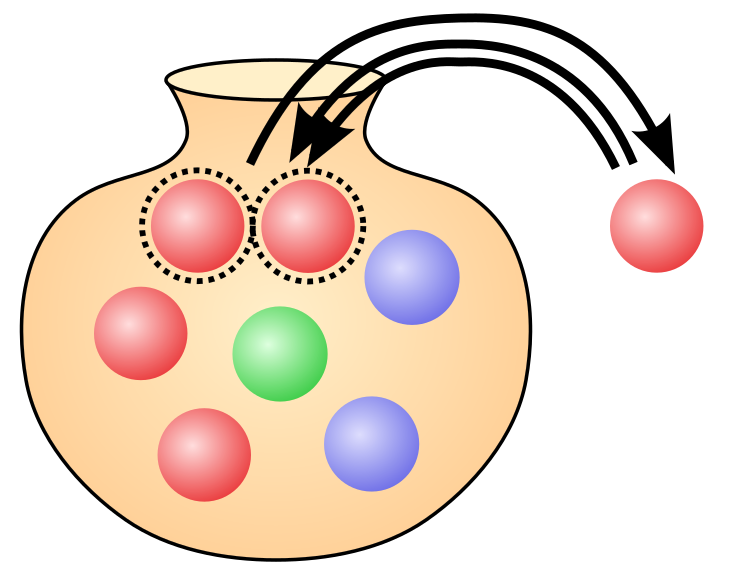
\includegraphics[width=\linewidth]{images/polya.png}
    \end{column}
    \begin{column}{0.6\linewidth}
      For simple example of the Spacey walk, consider P\'{o}lya Urn process.  Have urn with red and green balls inside, and repeat the following process:
      \begin{enumerate}
      \item Select a random ball from the urn
      \item Put the random ball back in the urn
      \item Put another ball of same selected color in the urn
      \end{enumerate}
    \end{column}
  \end{columns}
\end{frame}

% References
\begin{frame}
\frametitle{References}
\nocite*{}
\bibliographystyle{plain}
\bibliography{ho-markov}
\end{frame}

\end{document}
